\documentclass{article}

%% Denote paragraphs with vertical space rather than indenting (not critical)
\usepackage{parskip}

%% Support for URL in introductory text (not needed for main example)
\usepackage{url}

%% *** Enable TikZ ***
\usepackage{tikz}

%% *** TikZ library ***
\usetikzlibrary{math}

\begin{document}

%% Introductory Text
Example 4.11 from the book\\
\emph{Unlocking LaTeX Graphics: A Concise Guide to Ti$k$Z/PGF and PGFPLOTS}.\\
For more information, visit \url{https://latex-graphics.com}.
\par\bigskip

%% *** START OF EXAMPLE CODE ***
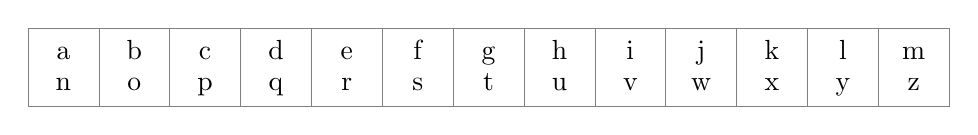
\begin{tikzpicture}[every node/.style={anchor=base},xscale=0.9]
  \draw[help lines] grid (13,1);
  \foreach[count=\cnt,
    evaluate=\cnt as \xx using {mod(\cnt-1,13)+0.5},
    evaluate=\cnt as \yy using {0.4*(1-div(\cnt-1,13))+0.2}
  ] \ltr in {a,b,...,z} { \node at (\xx,\yy) {\ltr}; }
\end{tikzpicture}
%% *** END OF EXAMPLE CODE ***

\end{document}
